\documentclass[tikz,border=4pt]{standalone}
\usepackage[T1]{fontenc}
\usepackage{lmodern}
\usetikzlibrary{arrows.meta,positioning,fit,backgrounds,calc}
\begin{document}
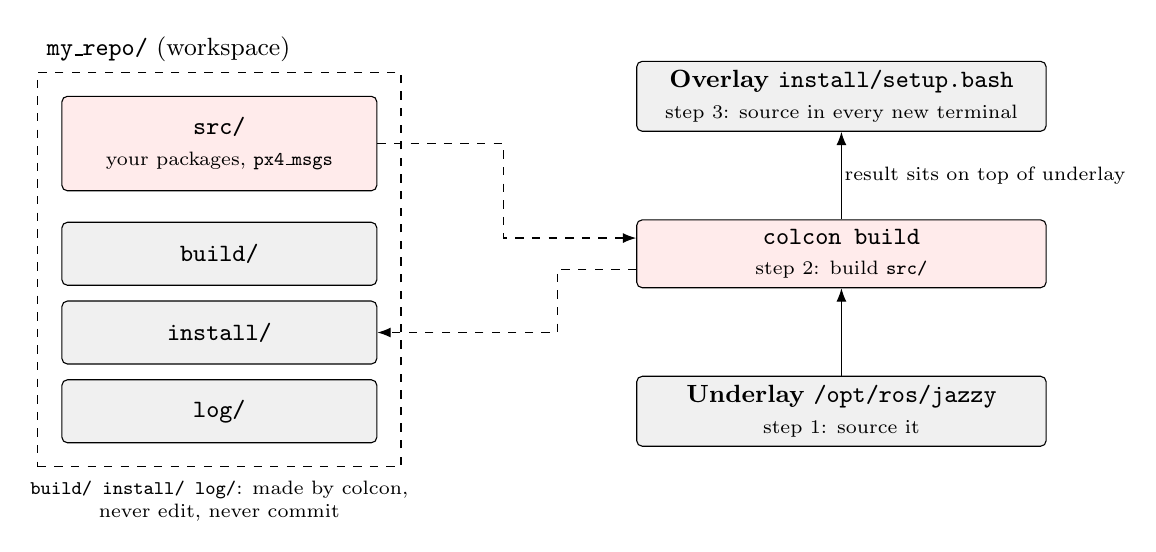
\begin{tikzpicture}[
  blk/.style={draw,rounded corners=2pt,minimum height=8mm,minimum width=40mm,align=center,font=\small,fill=white},
  ros/.style={blk,fill=red!8},
  ext/.style={blk,fill=gray!12},
  lab/.style={font=\scriptsize,fill=white,inner sep=1pt,align=center},
  >={Latex}]

\node[ros,minimum height=12mm] (src) at (2.3,-0.1) {\texttt{src/}\\\scriptsize your packages, \texttt{px4\_msgs}};
\node[ext] (build) at (2.3,-1.5) {\texttt{build/}};
\node[ext] (inst) at (2.3,-2.5) {\texttt{install/}};
\node[ext] (log) at (2.3,-3.5) {\texttt{log/}};
\begin{scope}[on background layer]
\node[draw,dashed,inner sep=3mm,fit=(src)(log)] (ws) {};
\end{scope}
\node[font=\small,anchor=south west] at (ws.north west) {\texttt{my\_repo/} (workspace)};
\node[lab,anchor=north] at (2.3,-4.35) {\texttt{build/ install/ log/}: made by colcon,\\never edit, never commit};
\node[ext,minimum width=52mm] (over) at (10.2,0.5) {\textbf{Overlay} \texttt{install/setup.bash}\\\scriptsize step 3: source in every new terminal};
\node[blk,minimum width=52mm,fill=red!8] (cb) at (10.2,-1.5) {\texttt{colcon build}\\\scriptsize step 2: build \texttt{src/}};
\node[ext,minimum width=52mm] (under) at (10.2,-3.5) {\textbf{Underlay} \texttt{/opt/ros/jazzy}\\\scriptsize step 1: source it};
\draw[->] (under) -- (cb);
\draw[->] (cb) -- node[lab,right]{result sits on top of underlay} (over);
\draw[->,dashed] (src.east) -- ++(1.6,0) |- ($(cb.west)+(0,0.2)$);
\draw[->,dashed] ($(cb.west)+(0,-0.2)$) -- ++(-1.0,0) |- (inst.east);

\end{tikzpicture}
\end{document}
